\section{Software testing}
\subsection{What is Software Testing}
\subsubsection{Bugs}
Ein Bug ist eine Schwachstelle im Programm, die ein inkorrektes Verhalten oder Ergebnis erzeugt. \newline
Warum bleiben Bugs im Programm:
\begin{itemize}
	\item Langes Testen ist teuer
	\item Veröffentlichungen hängen an Deadlines
	\item Eventuelle Konsequenzen, die am besten erst bei Major Releases eingeführt werden sollten
	\item Zu viele Releases nerven Nutzer
\end{itemize}
\subsubsection{Error}
Menschliche Aktivität erzeugt falsche Ergebnisse
\subsubsection{Fault}
System führt eine Funktion falsch aus
\subsubsection{Failure}
Abweichung des Ergebnisses vom erwarteten Ergebnis
\subsubsection{Validation}
Are we doing the right thing
\subsubsection{Verification}
Are we doing things rigth
\subsubsection{Inspection vs. Testing}
\begin{multicols}{2}
$\bold{Inspection}$	
\begin{itemize}
	\item Führt keinen Code aus und ist demnach nicht von Interaktionsfehlern betroffen
	\item Nicht gut, um Fehler in der Kommunikation zwischen Programmteilen zu erkennen
	\item Nicht vollständige Versionen können ohne weitere Kosten inspiziert werden
	\item Zusätzliche Suche nach Einhaltung von Standards, Tragbarkeit und Erhaltung
	\item Für kleine Unternehmen könnte ein separates Inspektionsteam zu teuer sein
\end{itemize}
\columnbreak
$\bold{Testing}$:
\begin{itemize}
	\item Manche Fehler können andere verbergen
	\item Gut, um Fehler in der Kommunikation zwischen Programmteilen zu erkennen
	\item Um unvollständigen Code zu Testen müssen extra Umgebungen entwickelt werden
\end{itemize}
\end{multicols}
\begin{table}[H]
\caption{Testing}
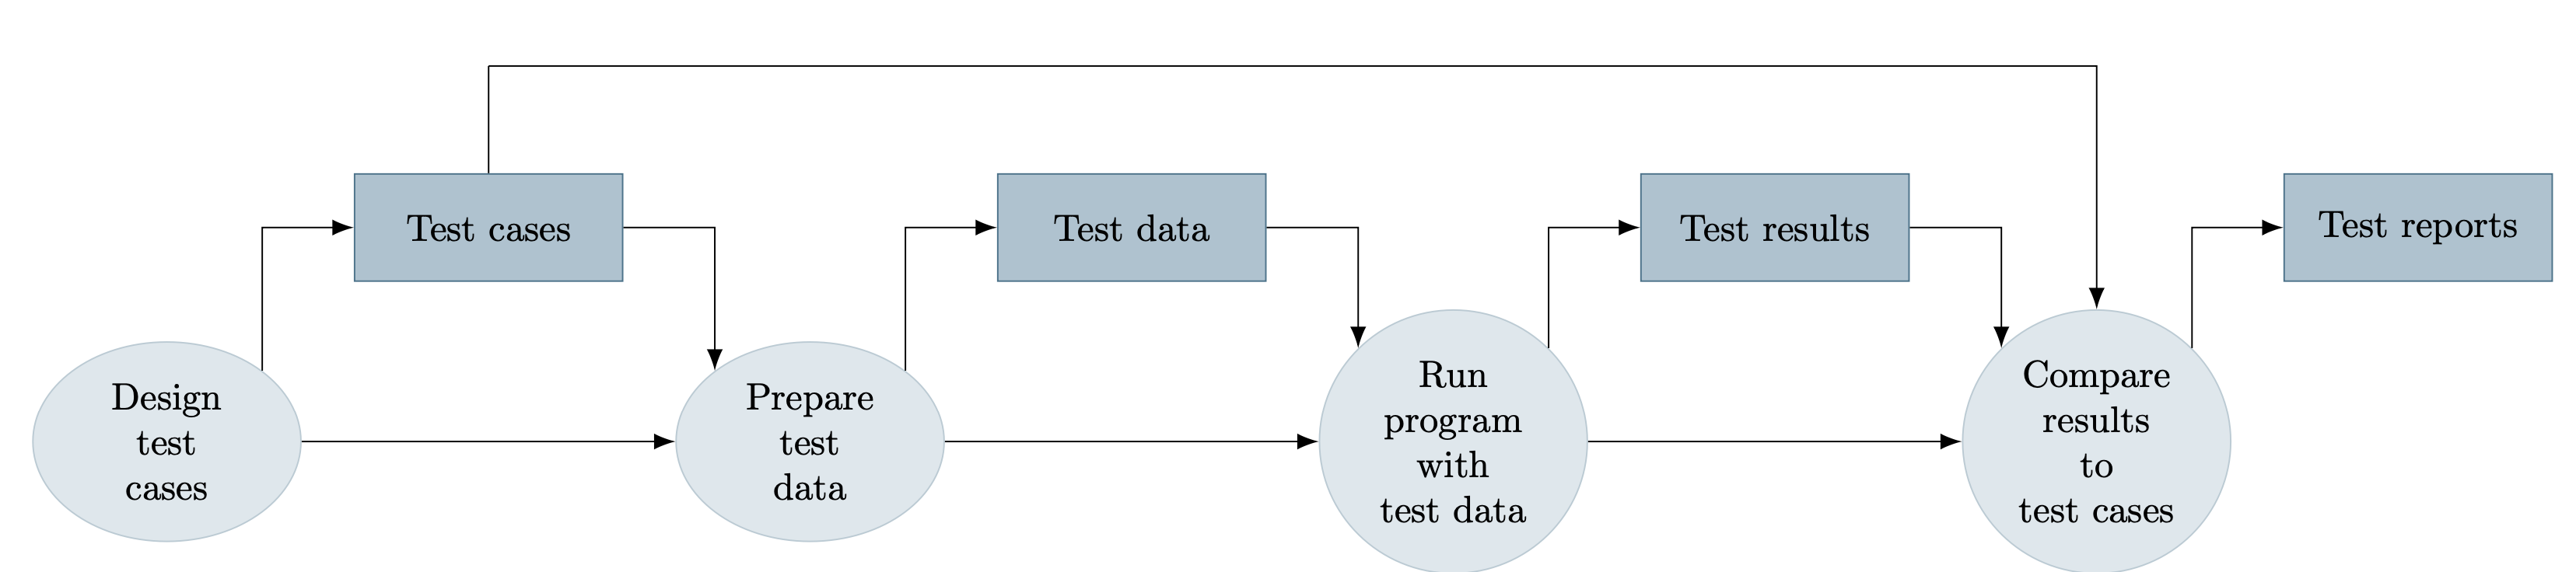
\includegraphics[scale=0.25]{Softweare_testing.png}	
\end{table}
\subsubsection{Stages of Software testing}
\begin{itemize}
	\item Development testing
		\begin{itemize}
			\item Um Bugs und Defekte zu entdecken
			\item Systemdesigners und Entwickler sind sehr wahrscheinlich beteiligt
		\end{itemize}
	\item Release testing
		\begin{itemize}
			\item Überprüfen, ob das System die Anforderungen erfüllt
			\item Ganzes System wird von einem separaten Team getestet
		\end{itemize}
	\item User testing
		\begin{itemize}
			\item Nutzer und potenzielle Nutzer testen das System in ihrer eigenen Umgebung
			\item z.B. acceptance testing
		\end{itemize}
\end{itemize}
\subsection{Development Testing}
\subsubsection{Unit Testing}
\begin{itemize}
	\item Teste individuelle Programmeinheiten oder Objektklassen
	\item Fokussiert sich auf Funktionalität
	\item Rufe die Funktionen oder Objekte mit verschiedenen Input-Parametern auf
	\item Teste alle Features der Objektklasse  
\end{itemize}
$\bold{Automated unit testing}$:
\begin{itemize}
	\item Setup part
	\item Call part
	\item Assertion part
\end{itemize}
$\bold{Mock objects}$:
\begin{itemize}
	\item Objekte können Abhängigkeiten zu externen Objekten haben, was das Testen ausbremst
	\item Mock objects haben das gleiche Interface, wie externe Objekte und simulieren ihre Funktionalität
	\item Mock objects können abnormale oder seltene Ereignisse simulieren
\end{itemize}
$\bold{Choosing}$ $\bold{unit}$ $\bold{tests}$:
\begin{itemize}
	\item Testfälle sollten zeigen, dass die getestete Komponente tut, was sie soll
	\item Testfälle sollten Defekte in der Komponente aufdecken
	\item Black-box testing: Testen, ohne näheres Wissen über die Komponente
\end{itemize}
\subsubsection{Component Testing}
\begin{itemize}
	\item Versucht zu testen, ob das Komponenteninterface funktioniert
	\item Geht davon aus, dass die einzelnen Komponenten der Komponente bereits die Unit tests bestanden haben
\end{itemize}
$\bold{Interface}$ $\bold{types}$:
\begin{itemize}
	\item Parameter interface: Daten oder Funktionen werden übergeben
	\item Shared memory interface: Ein Block an Daten wird geteilt
	\item Procedural interface: Eine Komponente kapselt ein set of procedures und kann von anderen aufgerufen werden
	\item Message passing interfaces: z.B. client-server 
\end{itemize}
$\bold{Interface}$ $\bold{errors}$:
\begin{itemize}
	\item Interface misuse
	\item Interface misunderstanding
	\item Timing errors
\end{itemize}
\subsubsection{System testing}
\begin{itemize}
	\item Testet das System im Ganzen
	\item Testet, ob Komponenten kompatibel sind und richtig interagieren
	\item Wird am besten von einem anderen Team durchgeführt
\end{itemize}
\subsection{Test-driven Development}
\begin{table}[H]
\caption{Test-driven development}
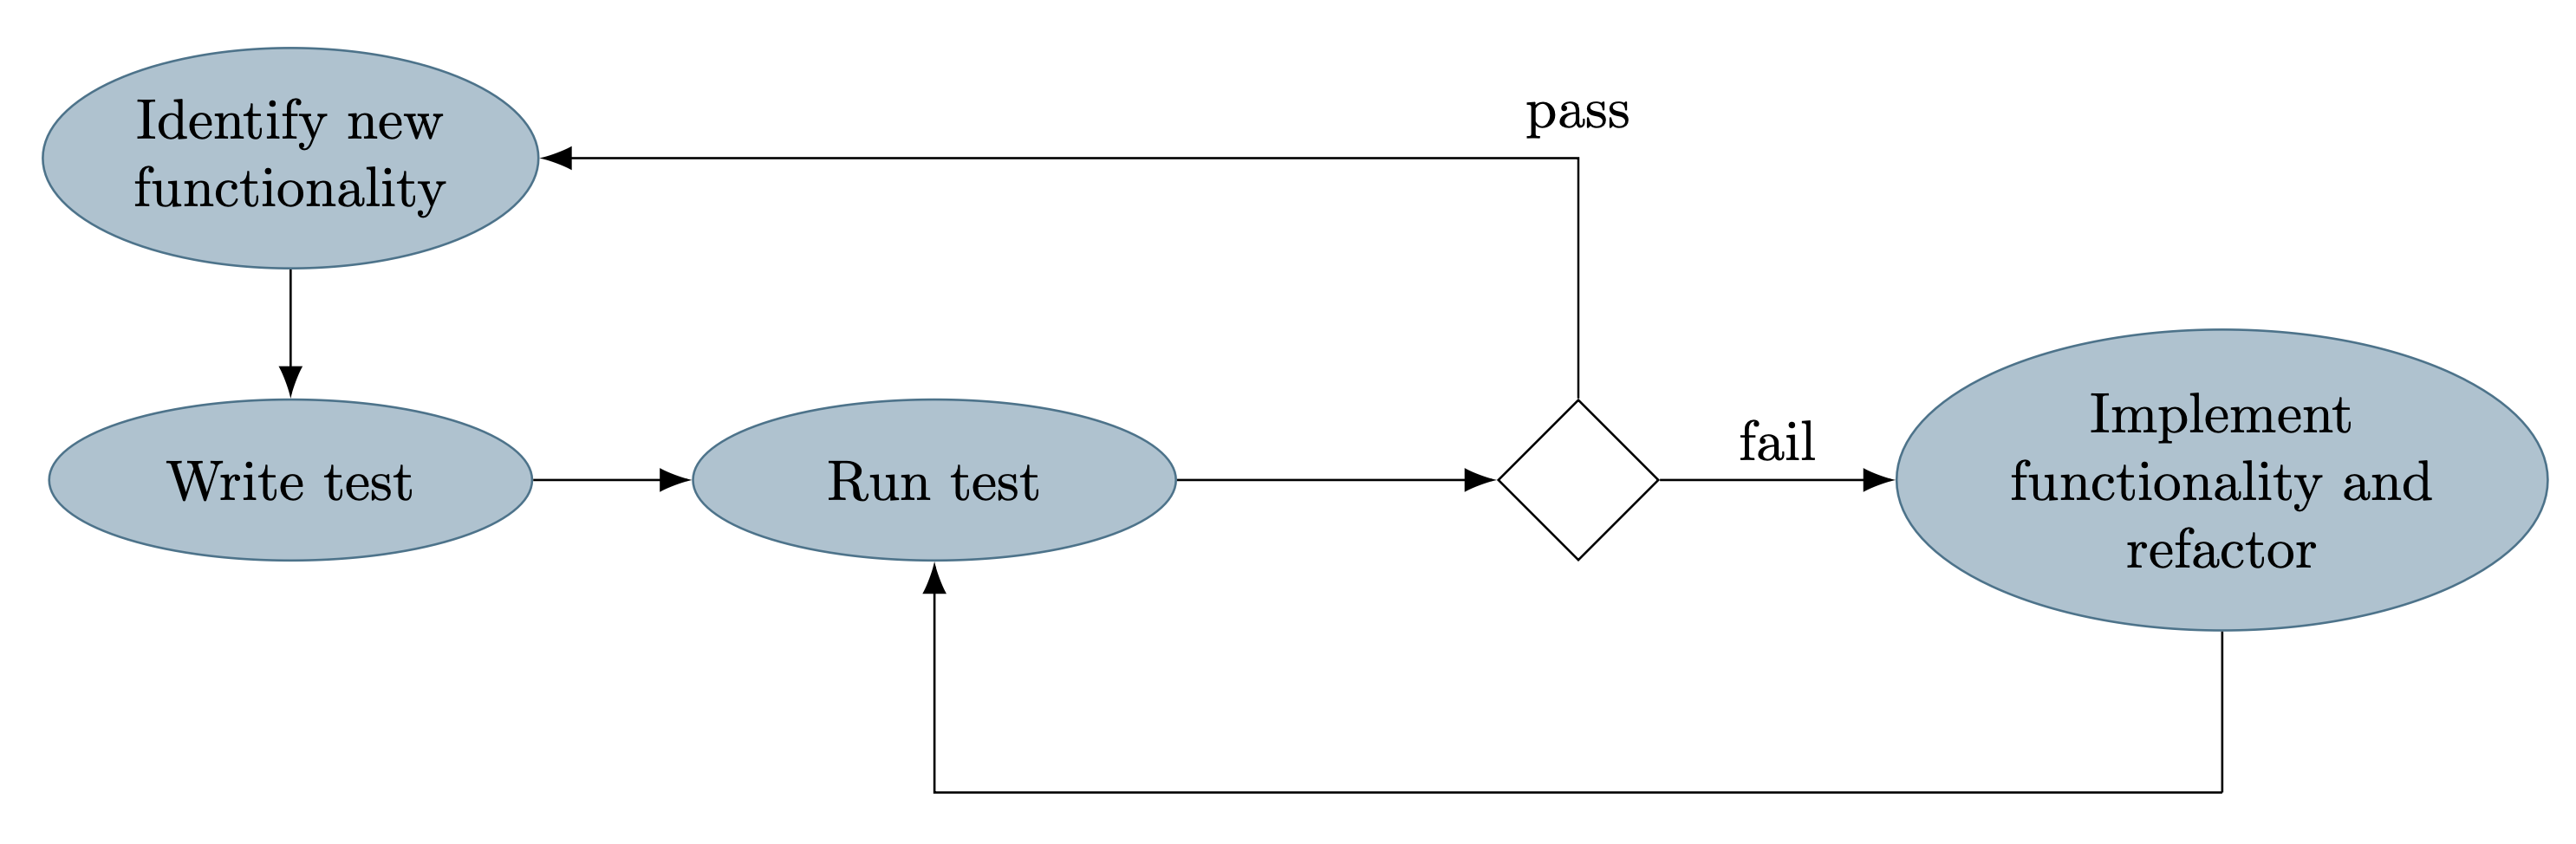
\includegraphics[scale=0.25]{TDD.png}
\end{table}
\begin{multicols}{2}
$\bold{Pros}$:
\begin{itemize}
	\item Hilft beim Verständnis, da der Test vorher geschrieben wird
	\item Jedes Codesegment hat einen Test
	\item Vereinfacht Debugging
	\item Test sind eine Form der Dokumentation
\end{itemize}
\columnbreak
$\bold{Cons}$:
\begin{itemize}
	\item Unpraktisch, beim Wiederverwenden von legacy code, da dieser im ganzen getestet werden muss
	\item Kann ineffektiv bei parallelen Systemen sein
\end{itemize}
\end{multicols}
\subsection{Releas Testing}
\begin{itemize}
	\item Das Entwicklungsteam sollte nicht daran beteiligt sein
	\item Validation checks müssen vorher überprüfen, ob die Software für Kunden bereit ist 
\end{itemize}
\subsubsection{Requirements-based testing‹}
\begin{itemize}
	\item Designe systematisch ein Set an Test-cases für jede Anforderung
	\item Validation check: Zeige, dass die Anforderungen korrekt umgesetzt wurden   
\end{itemize}
\subsubsection{Scenario testing}
\begin{itemize}
	\item Erzeuge ein typisches Szenario um Test-cases zu entwickeln
	\item Szenario:
		\begin{itemize}
			\item Realistisch
			\item Einfach zu evaluieren
			\item Stakeholders sollten sich damit identifizieren können
		\end{itemize}
\end{itemize}
\subsubsection{Performance testing}
\begin{itemize}
	\item Sichergehen, dass das System den die erwartete Last aushalten kann
	\item Sicherstellen, dass das System den Anforderungen entspricht
	\item Entdecke Probleme und Defekte im System
	\item Stresstests:
		\begin{itemize}
			\item Erhöhe die Last, bis das System zusammenbricht
			\item Teste das Verhalten bei einem Fehler: Zu hohe Ladung sollte keine Daten beschädigen
		\end{itemize}
\end{itemize}
\subsection{User Testing}
Die Umgebungen der Nutzer können Einfluss haben, auf:
\begin{itemize}
	\item Zuverlässigkeit
	\item Performance 
	\item Verwendbarkeit
	\item Stabilität
\end{itemize}
Es gibt drei Typen:
\begin{itemize}
	\item Alpha testing: Ausgewählte Gruppe
	\item Beta testing: Größere Gruppe
	\item Acceptance testing
\end{itemize}
\begin{table}[H]
\caption{User testing}	
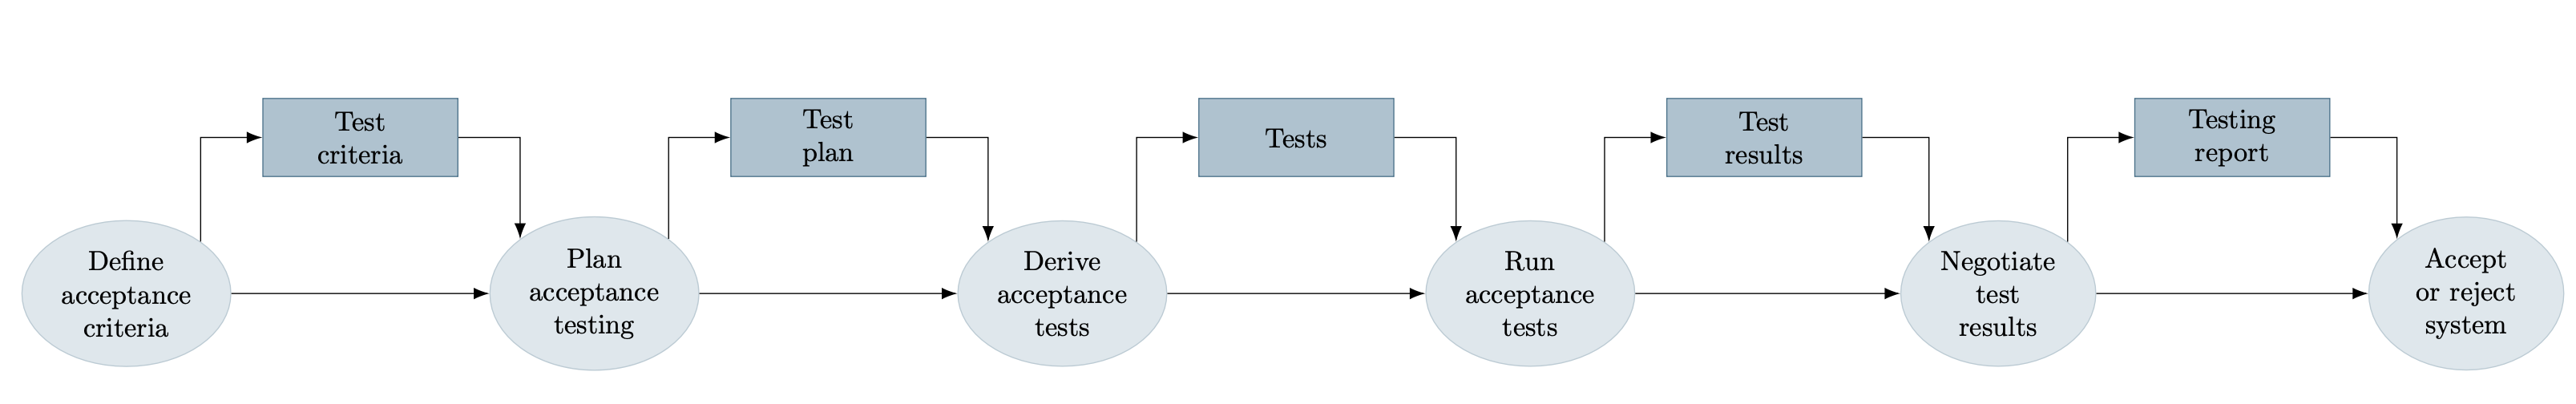
\includegraphics[scale=0.25]{User_testing.png}
\end{table}


